\documentclass[a4paper,12pt]{article}

%%%%%%%%%%%%%%%%%%%%%%%%%%%%%%%%%%%%%%%%%%%%%%%%
% Packages
%%%%%%%%%%%%%%%%%%%%%%%%%%%%%%%%%%%%%%%%%%%%%%%%

\usepackage[right=2.5cm, left=2.5cm, top=2.5cm, bottom=2.5cm]{geometry} 
\usepackage[portuguese]{babel}
\usepackage[T1]{fontenc}
\usepackage[utf8]{inputenc}
\usepackage{url}
\usepackage{hyperref}
\Urlmuskip=0mu  plus 10mu

% no indentation
%\usepackage{setspace}
%\setlength{\parindent}{0in}

\usepackage{graphicx} 
\usepackage{float}
\usepackage{xcolor}

\usepackage{mathtools}
\usepackage{amssymb, amsthm}

% headers
\usepackage{fancyhdr}

%%%%%%%%%%%%%%%%%%%%%%%%%%%%%%%%%%%%%%%%%%%%%%%%
% Proper definitions
%%%%%%%%%%%%%%%%%%%%%%%%%%%%%%%%%%%%%%%%%%%%%%%%
\newcommand{\R}{\mathbb{R}}

\newtheoremstyle{exer}{}{}{\color{blue}}{}{\color{blue}\bfseries}{}{ }{}
\theoremstyle{exer}
\newtheorem{exercise}{Exercício}

\theoremstyle{definition}
\newtheorem{solution}{Solução}

\theoremstyle{plain}
\newtheorem{remark}{Observação}



%%%%%%%%%%%%%%%%%%%%%%%%%%%%%%%%%%%%%%%%%%%%%%%%
% Header (and Footer)
%%%%%%%%%%%%%%%%%%%%%%%%%%%%%%%%%%%%%%%%%%%%%%%%

\pagestyle{fancy} 
\fancyhf{}

\lhead{\footnotesize CS: Lista 4}
\rhead{\footnotesize Prof. Asla e Mon. Lucas} 
\cfoot{\footnotesize \thepage} 


\begin{document}

%%%%%%%%%%%%%%%%%%%%%%%%%%%%%%%%%%%%%%%%%%%%%%%%
% Title section of the document
%%%%%%%%%%%%%%%%%%%%%%%%%%%%%%%%%%%%%%%%%%%%%%%%

\thispagestyle{empty} 

\begin{tabular*}{0.95\textwidth}{l @{\extracolsep{\fill}} r} 
    {\large \bf Curvas e Superfícies 2022.1} &  \\
    Escola de Matemática Aplicada, Fundação Getulio Vargas &  \\
    Professora Asla Medeiros e Sá &  \\ 
    Monitor Lucas Machado Moschen & Entrega 13/04/2022\\
    \hline \\
\end{tabular*} 
\vspace*{0.3cm} 

\begin{center}
	{\Large \bf Lista 4}
	\vspace{2mm}
\end{center}  
\vspace{0.4cm}

\begin{exercise}
    Verifique se as seguintes curvas são 2-regulares:
    \begin{enumerate}
        \item[(a)] $\alpha(t) = (t, t^2, t^3), t \in \R$
        \item[(b)] $\alpha(t) = (t, t^2 + 2, t^3 + t), t \in \R$
    \end{enumerate}
\end{exercise}

\begin{solution}
    De forma geral, para conferir que uma curva é regular de ordem $m$,
    pedimos que os vetores correspondentes às primeiras $m$ derivadas sejam
    linearmente independentes\footnote{Wikipedia:
    \url{https://en.wikipedia.org/wiki/Differentiable_curve\#Definitions}}. Se
    a curva é parametrizada pelo comprimento de arco, a primeira e a segunda
    derivadas são ortogonais e, portanto, linearmente independentes. Como as
    funções acima tem segunda derivada com 0 na primeira componente, mas tem
    valor 1 na primeira, basta verificar que $\alpha ''(t) \neq 0$. 
    \begin{enumerate}
        \item[(a)] $\alpha''(t) = (0,2,6t) \neq 0 \forall t \in \R$
        \item[(b)] $\alpha''(t) = (0,4,6t) \neq 0 \forall t \in \R$  
    \end{enumerate}
\end{solution}

\begin{exercise}
    Prove que a aplicação $\alpha(t) = (1 + \cos(t), \sin(t), 2\sin(t/2)), t
    \in \R$, é uma curva regular cujo traço está contido na interseção do
    cilindro $C = \{(x, y, z) \in \R^3; (x - 1)^2 + y^2 = 1\}$ e da esfera $S
    = \{(x, y, z) \in \R^3; x^2 + y^2 + z^2 = 4\}$. Desenhe a curva $\alpha$,
    o cilindro $C$ e a esfera $S$ em ambiente computacional.    
\end{exercise}

\begin{solution}
    Primeiro vamos provar que a curva é regular. Derivando obtemos:
    $$
    \alpha '(t) = (-\sin(t), \cos(t), \cos(t/2)),
    $$
    como $\sin(t)^2 + \cos^2(t) = 1$, se um deles for nulo, o outro
    obrigatoriamente não será e $\alpha$ é regular. Para mostrar que o traço
    está contido nessa interseção, tome $t \in \R$ e defina $(x,y,z) :=
    \alpha(t)$. Assim: 
    $$
    (x - 1)^2 + y^2 = cos^2(t) + \sin^2(t) = 1
    $$
    o que implica que $(x,y,z) \in C$. Além disso, 
    $$
    x^2 + y^2 + z^2 = 1 + 2\cos(t) + \cos^2(t) + \sin^2(t) + 4\sin^2(t/2) = 2(1 + \cos(t)) + 4\sin^2(t/2)
    $$
    Como $\cos(t) = \cos^2(t/2) - \sin^2(t/2) = 2\cos^2(t/2) - 1$, temos que 
    $$
    x^2 + y^2 + z^2 = 4\cos^2(t/2) + 4\sin^2(t/2) = 4
    $$
    o que implica $(x,y,z) \in S$. Como $t$ é arbitrário, o traço da curva
    está contido na intersecção. Confira a Figura \ref{fig-exer2}.

    \begin{figure}
        \centering
        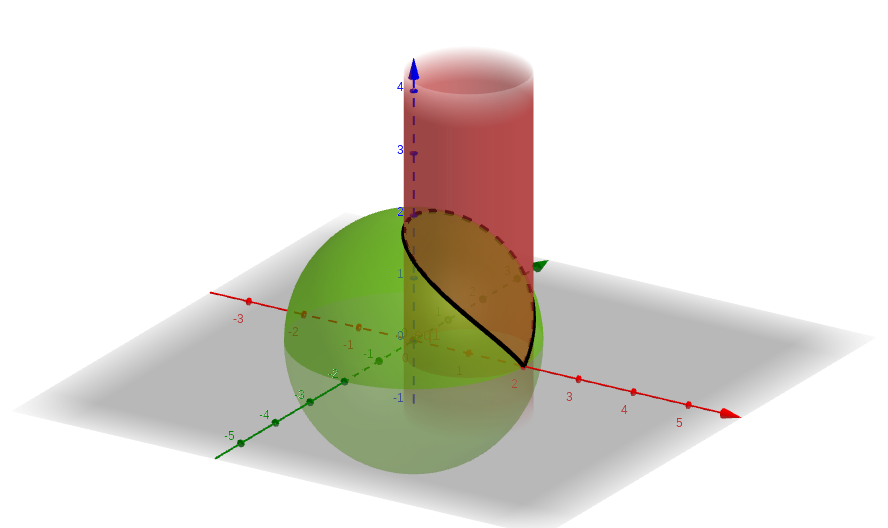
\includegraphics[width=0.7\textwidth]{images/exer2.png}
        \caption{Intersecção de cilindro e esfera. Arquivo está no Github.}
        \label{fig-exer2}
    \end{figure}
\end{solution}

\begin{exercise}
    Obtenha uma reparametrização por comprimento de arco da curva
    $$\alpha(t) = (e^t\cos(t), e^t\sin(t), e^t), t \in \R$$
\end{exercise}

\begin{solution}
    Para obter uma reparametrização pelo comprimento de arco, primeiro
    precisamos encontrar a função comprimento de arco. 
    $$
    \alpha'(t) = e^t(\cos(t) - \sin(t), \cos(t) + \sin(t), 1)
    $$
    Assim
    $$
    L_0^t(\alpha) = \int_0^t ||\alpha'(s)||ds = \int_0^t e^s\sqrt{3}ds = \sqrt{3}e^t - \sqrt{3}
    $$
    Assim defina $g(t) = \sqrt{3}e^t$. Sabemos que essa transformação é um
    difiomorfismo e que se $\beta(s) = \alpha(g^{-1}(s))$, teremos que $\beta$
    será parametrizada pelo comprimento de arco. Como 
    $$
    g^{-1}(s) = \log\left(\frac{s}{\sqrt{3}}\right)
    $$
    Uma parametrização pelo comprimento arco é 
    $$
    \beta(s) = \frac{s}{\sqrt{3}}\left(\cos(\log(s/\sqrt{3})), \sin(\log(s/\sqrt{3})), 1\right)
    $$
\end{solution}

\begin{exercise}
    Seja $\alpha : I \to \R^3$ uma curva regular. Prove que $||\alpha'(t)||$ é
    constante se, e só se, $\forall t \in I, \alpha''(t)$ é ortogonal a
    $\alpha'(t)$. Em particular, mostre que $||\alpha'(t)||$ é constante para a hélice circular $\alpha(t) = (a\cos(t), a\sin(t), b.t), t \in R$.
\end{exercise}

\begin{solution}
    Lembre que $||\alpha '(t)||^2 = \langle \alpha '(t), \alpha'(t) \rangle$.
    Assim, para todo $t$ 
    $$
    k^2 = \langle \alpha '(t), \alpha'(t) \rangle \iff \frac{d}{dt}\langle \alpha '(t), \alpha'(t) \rangle = 2\langle \alpha '(t), \alpha''(t) \rangle = 0 \iff \alpha'(t) \perp \alpha''(t)
    $$
    No caso da  hélice, observe que 
    $$
    \alpha'(t) = (-a\sin(t), a\cos(t), b)
    $$
    $$
    \alpha''(t) = (-a\cos(t), -a\sin(t), 0)
    $$
    Assim $\langle \alpha '(t), \alpha ''(t) \rangle = 0 \implies
    ||\alpha'(t)||$ é constante. 
\end{solution}

\begin{exercise}
    Em ambiente computacional, desenhe as seguintes curvas e produza uma
    animação do triedro de Frenet de cada curva:
    \begin{enumerate}
        \item[(a)] $\alpha(t) = (4\cos(t), 5 - 5\sin(t), - 3\cos(t)), t \in \R
        \in \R$
        \item [(b)] $\beta(t) = (1 - \cos(t), \sin(t), t), t \in \R$
    \end{enumerate}
\end{exercise}

\begin{solution}
    Nesse exercício, é importante parametrizarmos pelo comprimento de arco,
    porque definimos o Triedo de Frenet apenas dessa forma (por enquanto). No
    desenho, eu multipliquei os vetores unitários por uma constante $k$ para
    que eles ficassem visíveis quando comparados com a curva. O desenho de (a) está no
    Geogebra e (b) é equivalente. Confira a Figura \ref{fig-exer5}.

    \begin{figure}
        \centering
        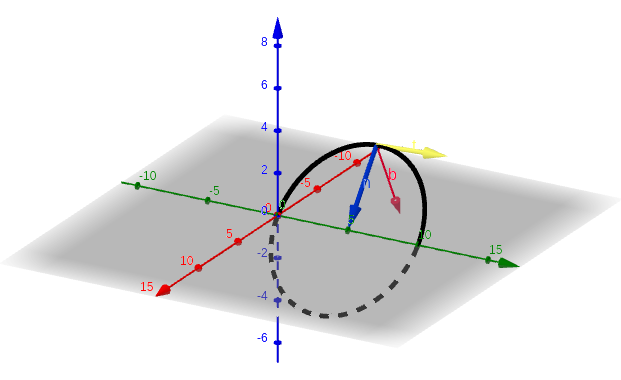
\includegraphics[width=0.7\textwidth]{images/exer5-a.png}
        \caption{Triedo de Frenet de uma circunferência.}
        \label{fig-exer5}
    \end{figure}
\end{solution}

\begin{exercise}
    Seja $\alpha : I \to \R^3$ uma curva 2-regular, a qual, não é,
    necessariamente, parametrizada por comprimento de arco. Prove, então, que 
    $$\kappa_{\alpha}(t) = \frac{||\alpha'(t) \times \alpha''(t)||}{||\alpha'(t)||^3}$$
    $$\tau_{\alpha}(t) = \frac{\langle \alpha'(t) \times \alpha''(t),\alpha'''(t) \rangle}{||\alpha'(t) \times \alpha''(t)||^2}$$
    em que $\times$ denota o produto vetorial.
\end{exercise}

\begin{solution}
    Para esse exercício, vale consultar o livro \cite{pressley}, em especial a
    Proposição 2.1.2 na página 31 e a Proposição 2.3.1 na página 48.
\end{solution}

\begin{exercise}
    Calcule a curvatura e a torção das seguintes curvas:
    \begin{enumerate}
        \item[(a)] $\alpha(t) = (t, t^2, t^3), t \in R$
        \item[(b)] $\beta(t) = (\cos(t), \sin(t), t), t \in R$
    \end{enumerate}
\end{exercise}

\begin{solution}
    A ideia desses exercícios é usar as fórmulas demonstradas no exercício
    passado:
    \begin{enumerate}
        \item[(a)] Primeiro calculamos as três derivadas
        $$
        \alpha'(t) = (1,2t,3t^2)
        $$
        $$
        \alpha''(t) = (0,2,6t)
        $$
        $$
        \alpha'''(t) = (0,0,6)
        $$
        Agora calculemos algumas expressões
        $$
        \alpha'(t) \times \alpha''(t) = (6t^2, -6t, 2)
        $$
        $$
        ||\alpha'(t) \times \alpha''(t)||^2 = 36t^4 + 36t^2 + 4
        $$
        Usando as fórmulas, 
        $$
        \kappa_{\alpha}(t) = \sqrt{\frac{36t^4 + 36t^2 + 4}{(1 + 4t^2 + 9t^4)^3}}
        $$
        $$
        \tau_{\alpha}(t) = \frac{3}{9t^4 + 9t^2 + 1}
        $$
        \item[(b)] Primeiro calculamos as três derivadas
        $$
        \alpha'(t) = (-\sin(t),\cos(t),1)
        $$
        $$
        \alpha''(t) = (-\cos(t),-\sin(t),0)
        $$
        $$
        \alpha'''(t) = (\sin(t),-\cos(t),0)
        $$
        Agora calculemos algumas expressões
        $$
        \alpha'(t) \times \alpha''(t) = (\sin(t),-\cos(t),1)
        $$
        $$
        ||\alpha'(t) \times \alpha''(t)||^2 = 2
        $$
        Usando as fórmulas, 
        $$
        \kappa_{\alpha}(t) = \frac{2^{1/2}}{2^{3/2}} = \frac{1}{2}
        $$
        $$
        \tau_{\alpha}(t) = \frac{1}{2}
        $$
    \end{enumerate}
\end{solution}

\begin{exercise}
    Seja $\alpha(t)$ uma curva 2-regular:
    \begin{enumerate}
        \item[(a)] Verifique que $\alpha''(t)$ é paralelo ao plano osculador de $\alpha$ em $t$.
        \item[(b)] Prove que o plano osculador de $\alpha$ em $t_0$ é dado
        pelos pontos $P$ de $R^3$ tal que $\langle P - \alpha(t_0), \alpha
        '(t_0) \times \alpha''(t_0) \rangle = 0$
    \end{enumerate}
\end{exercise}

\begin{solution}
    Assim
    \begin{enumerate}
        \item[(a)] O plano osculador é gerado pelos vetores tangente e normal
        à curva $\alpha$ a cada $t$. Considere $\beta = \alpha \circ \phi$ a parametrização de
        $\alpha$ pelo comprimento de arco. Temos que $\dot{\beta}(s)$ e
        $\ddot{\beta}(s)/\kappa_{\beta}(s)$ geram o plano osculador e,
        portanto, $\ddot{\beta}(s)$ e $\dot{\beta}(s)$ são paralelos ao plano osculador. Ainda
        $$
        \dot{\beta}(s) = \dot{\alpha}(\phi(s))\cdot\dot\phi(s) 
        $$
        o que implica $\dot{\alpha}(t)$ ser paralelo ao plano osculador. Além
        disso, 
        $$
        \ddot{\beta}(s) = \ddot{\alpha}(\phi(s))\cdot(\dot{\phi}(s))^2 + \dot{\alpha}(\phi(s))\cdot\ddot\phi(s) \implies \ddot{\alpha}(\phi(s))\cdot(\dot{\phi}(s))^2 = \ddot{\beta}(s) - \dot{\alpha}(\phi(s))\cdot\ddot\phi(s) 
        $$
        Concluo que $\ddot\alpha(t)$ é paralelo ao plano osculador, pois é
        paralelo à soma de vetores paralelos. 

        \item[(b)] Sabemos que o plano osculador é dado pelos pontos $P$ tal
        que $\langle P - \alpha(t_0), B(t) \rangle = 0$, onde $B(t)$ é o vetor
        binormal. Usando um raciocínio similar ao exercício 6,
        conseguimos provar que 
        $$
        B(t) = \frac{\dot\alpha \times \ddot\alpha}{||\dot\alpha \times \ddot\alpha||} 
        $$
        e, portanto, está provado.
    \end{enumerate}
\end{solution}

\begin{exercise}
    Desenhe em ambiente computacional as curvas e seus planos normal e
    osculador em função do parâmetro:
    \begin{enumerate}
        \item[(a)] $\alpha(t) = (3t - t^3, 3t^2, 3t + t^3), t \in R$.
        \item[(b)] $\beta(t) = (a\cos(t) + b\sin(t), a\sin(t) + b\cos(t), c\sin(2t)), t \in R$.
    \end{enumerate}
\end{exercise}

\begin{solution}
    Solução a cargo do leitor. 
\end{solution}

\begin{exercise}
    Verifique que o vetor binormal de uma hélice circular forma um ângulo
    constante com o eixo do cilindro sobre o qual está a hélice. Ilustre o
    fato em ambiente computacional.
\end{exercise}

\begin{solution}
    Considere a hélice circular 
    $$
    \hat{\gamma}(t) = (a\cos(t), a\sin(t), bt)
    $$
    A norma da derivada é dada por $\sqrt{a^2 + b^2} := c$. Assim, podemos
    reparametrizar pelo comprimento de arco, 
    $$
    \gamma(t) = (a\cos(t/c), a\sin(t/c), bt/c)
    $$
    Primeiro calculamos os vetores tangente e normal,
    $$
    T(t) = \frac{1}{c}(-a\sin(t/c), a\cos(t/c), b)
    $$
    $$
    \dot{T}(t) = -\frac{a}{c^2}(\cos(t/c), \sin(t/c), 0)
    $$
    $$
    N(t) =  (-\cos(t/c), -\sin(t/c), 0)
    $$
    E agora o binormal, 
    $$
    B(t) = T(t) \times N(t) = \frac{1}{c}(b\sin(t/c), -b\cos(t/c), a) 
    $$
    O eixo do cilindro que a hélice se encontra é gerado pelo vetor $e_3 =
    (0,0,1)$. E 
    $$
    \langle B(t), e_3 \rangle = a, \forall t \in \R 
    $$
    Assim, o cosseno do ângulo formado por esses dois vetores é constante e,
    definindo o ângulo entre dois vetores entre $[0,\pi]$, teremos ângulo
    constante. 
\end{solution}

\begin{exercise}
    Prove que a aplicação
    $$\alpha(s) = \left(\frac{4}{5}\cos(s), 1 - \sin(s), -\frac{3}{5}\cos(s)\right), s
    \in \R$$
    é uma curva regular, parametrizada por comprimento de arco, cujo traço é um círculo.
    Determine, então, seus centro e raio.
\end{exercise}

\begin{solution}
    Veja que $\alpha'(s) = \left(-\frac{4}{5}\sin(s), -\cos(s),
    \frac{3}{5}\sin(s)\right)$ e, portanto
    $$
    ||\alpha'(s)||^2 = \frac{16}{25}\sin^2(s) + \cos^2(s) + \frac{9}{25}\sin^2(s) = 1
    $$
    portanto $\alpha$ é uma curva regular, parametrizada pelo comprimento de
    arco. Agora observe que 
    $$
    \alpha''(s) = \left(-\frac{4}{5}\cos(s), \sin(s). \frac{3}{5}\cos(s)\right) \implies \kappa_{\alpha}(s) = 1
    $$
    Usando a fórmula para a torção, encontramos que 
    $$
    \tau_{\alpha} = -\frac{1}{5}(3,0,4)\cdot\left(\frac{4}{5}\sin(s), \cos(s), -\frac{3}{5}\sin(s)\right) = 0
    $$
    Como a torção é nula, nossa curva está num plano. Como a curvatura é
    constante, pelo Teorema Fundamental das Curvas no Plano, ela é igual a um
    círculo após um movimento rígido. Todavia, provamos na última lista que
    movimento rígido transforma círculos em círculos. Portanto nossa curva é
    um círculo. Em particular encontrar que o raio é 1. Por fim, observe que 
    $$
    ||\alpha(s) - (0,1,0)||^2 = \frac{16}{25}\cos^2(s) + \sin^2(s) + \frac{9}{25}\cos^2(s) = 1 
    $$
    o que mostra que o centro é dado por $(0,1,0)$. 
\end{solution}

\begin{thebibliography}{9}
    \bibitem{pressley} 
    Pressley, Andrew N. Elementary differential geometry. Springer Science \& Business Media, 2010.
\end{thebibliography}

\end{document}